%"###############################################
%
% Corrélations 
%
%###############################################

Ici nous souhaitons mettre en évidence les corrélations possibles.
Nous limitons l’étude sur les tableaux post-opératoires des techniques RTUBD VPPBS et VAPOR contenant 
aussi les variables IPSS Qol et Qmax.
De même, certaines dimensions sont invariantes pour une technique donnée, nous avons supprimé celles-ci lors de la création 
de la matrice de corrélation et son corralélograme associé.

\begin{figure}[H]
\centering
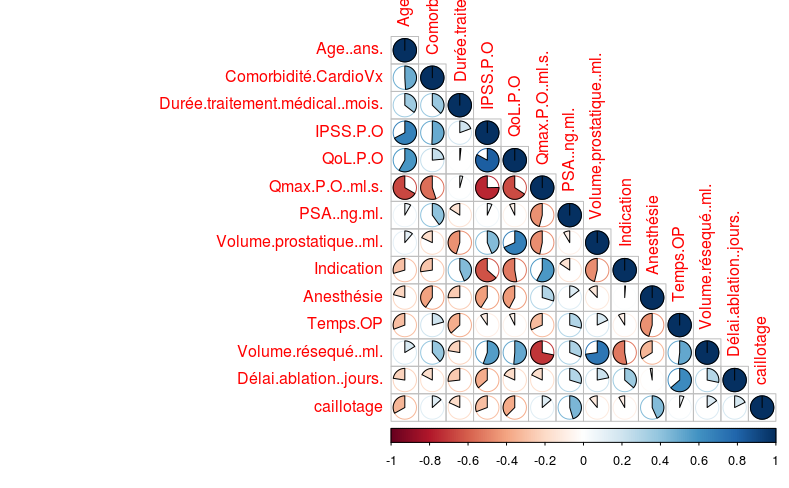
\includegraphics[width=0.75\textwidth]{../Fig/RTUPB/rtupb-corr-matrice-pie}
\caption{Matrice corrélation RTUBP}
\end{figure}

\begin{figure}[H]
\centering
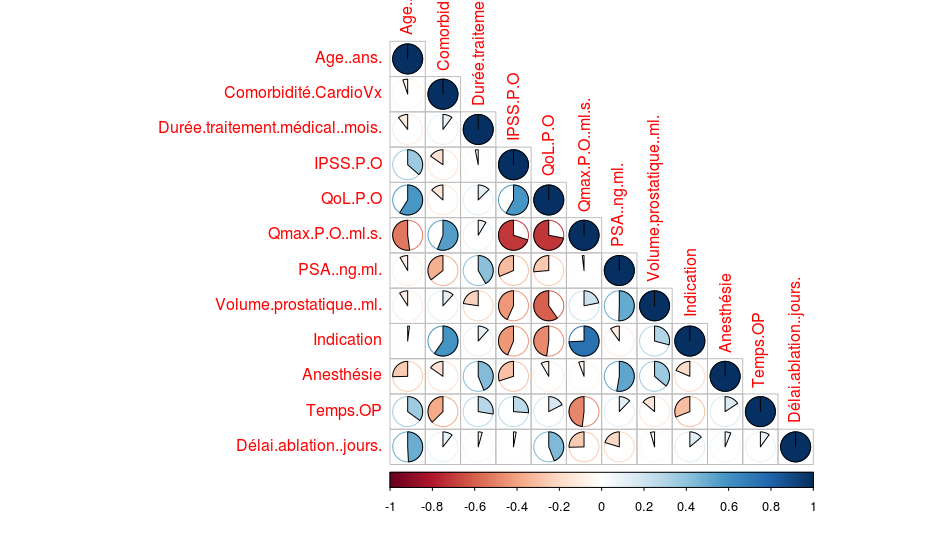
\includegraphics[width=0.75\textwidth]{../Fig/VPPBS/vppbs-corr-matrice-pie}
\caption{Matrice corrélation VPPBS}
\end{figure}

\begin{figure}[H]
\centering
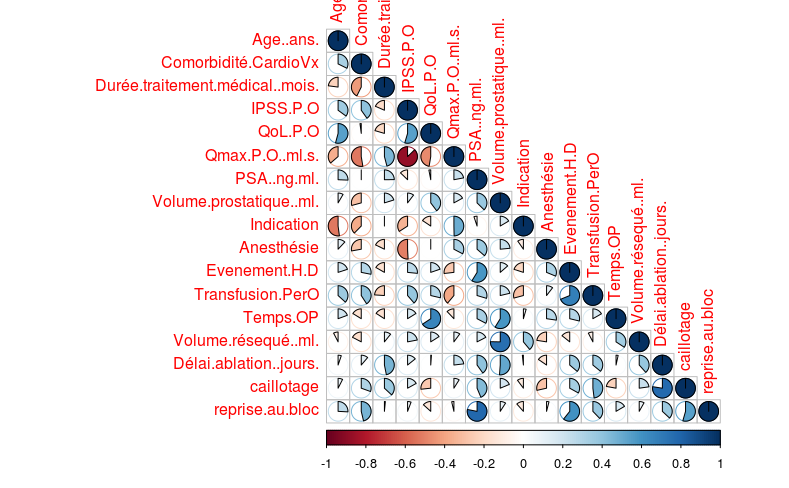
\includegraphics[width=0.75\textwidth]{../Fig/VAPOR/vapor-corr-matrice-pie}
\caption{Matrice corrélation VAPOR}
\end{figure}


Les variables  \emph{IPSS P.O} et   \emph{QoL P.O}  semblent avoir une corrélation qui peut sembler logique à la connaissance du fait qu’elles représentent pour l’une un indicateur de gêne et pour l’autre un indicateur une qualité de vie post opératoire, même si c’est nettement plus marqué dans le cas du panel des patients RTUPB. De même  pour les variables \emph{Volume prostatique} et \emph{Volume réséqué}. Aussi nous avons une corrélation \textbf{négative} intéressante entre le \emph{IPSS P.O} et le \emph{QMAX PO (ml/s)} (plus le patient à un QMax élevé moins il semble gêné alors que IPSS croît avec la gêne). 




%\begin{figure}[h]
%    \begin{minipage}[c]{.46\linewidth}
%        \centering
%        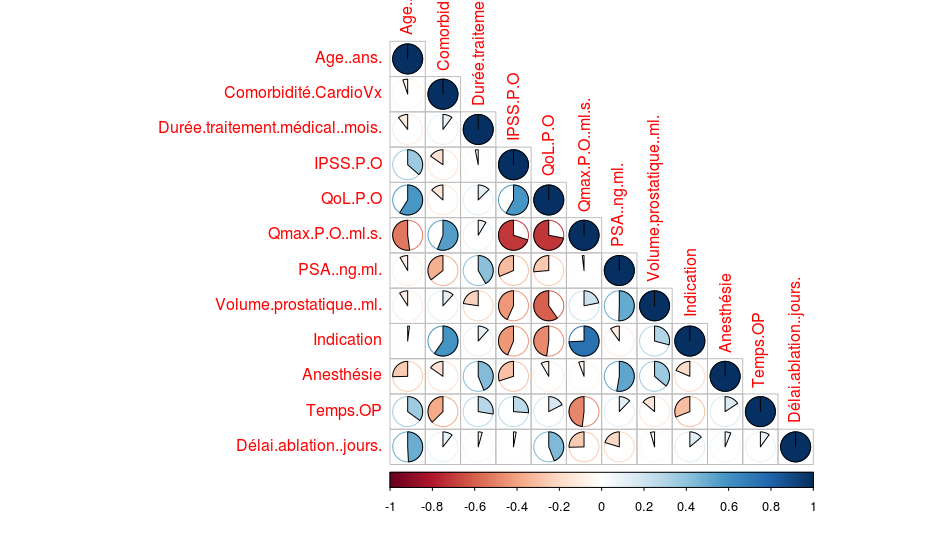
\includegraphics[width=1\textwidth]{../Fig/VPPBS/vppbs-corr-matrice-pie}
%        \caption{Légende}
%    \end{minipage}
%    \hfill%
%    \begin{minipage}[c]{.46\linewidth}
%        \centering
%        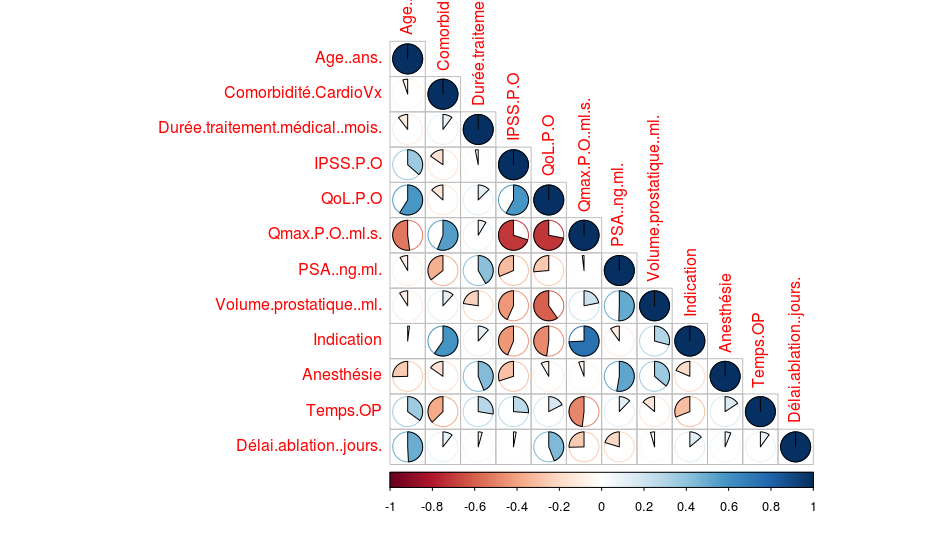
\includegraphics[width=1\textwidth]{../Fig/VPPBS/vppbs-corr-matrice-pie}
%        \caption{Légende}
%    \end{minipage}
%\end{figure}





%
%##########################
%# CONCLUSION
%##########################